\section{Can the model find the right articulation?}
\label{sec:articulation}

\begin{figure}[!htb]
\centering
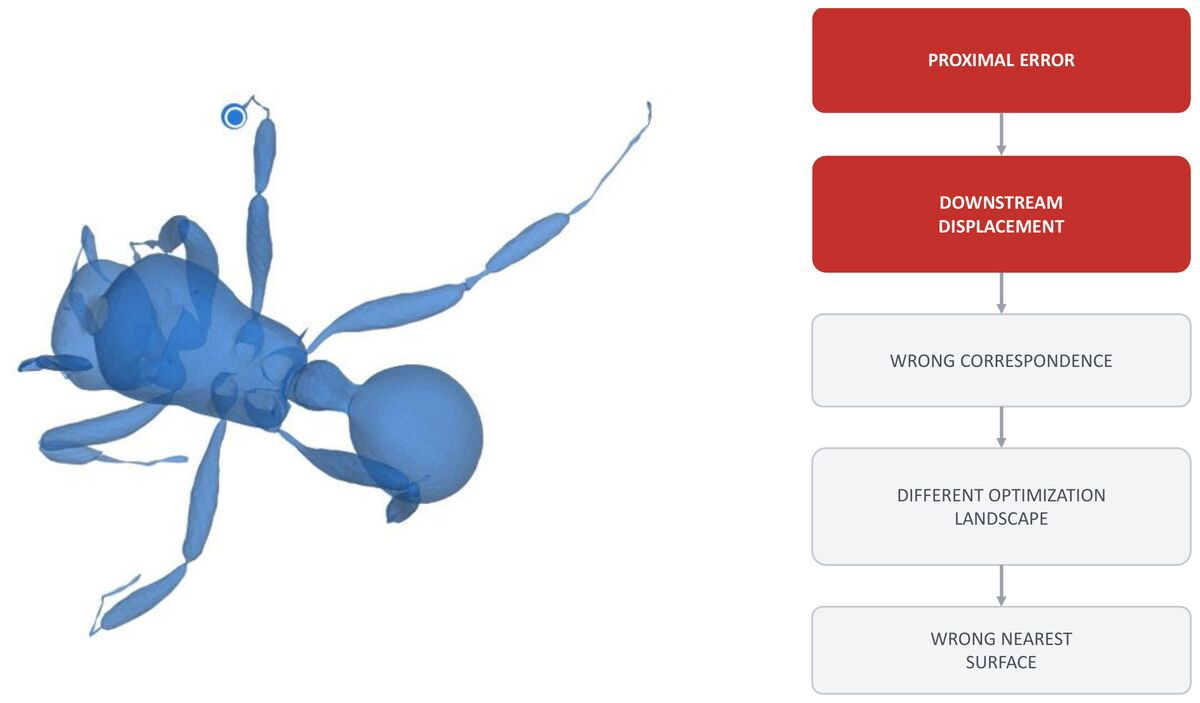
\includegraphics[width=0.62\linewidth]{figures/fig_articulation_flow.jpg}
\caption{A pose error near the body (proximal) propagates downstream through
the kinematic chain, so the vertex most likely to end up mis-corresponded is
not the one where the error originated but everything distal to it.}
\label{fig:articulation-flow}
\end{figure}

\begin{figure}[!htb]
\centering
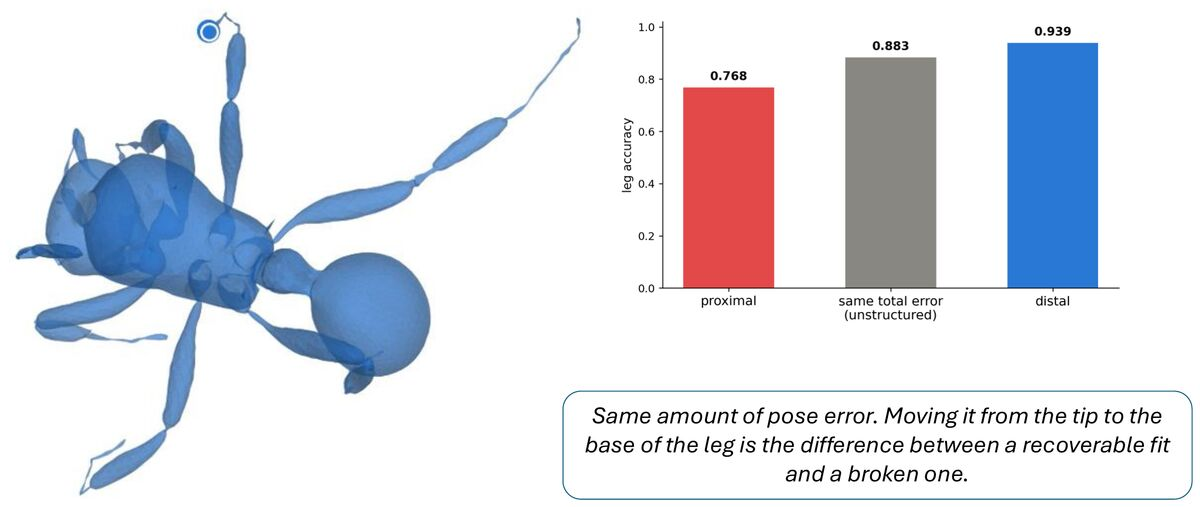
\includegraphics[width=0.5\linewidth]{figures/fig_articulation_bars.jpg}
\caption{Leg accuracy for the same total amount of pose error, placed at
different points along the kinematic chain. Moving an identical error budget
from the tip (distal) to the base (proximal) of the leg is the difference
between a recoverable fit (0.94) and a badly broken one (0.77).}
\label{fig:articulation-bars}
\end{figure}

\begin{investigation}{I4}{Is initialisation sensitivity uniform along the kinematic chain?}
\invQuestion{Does starting the optimiser from the ground-truth pose recover
the accuracy lost under default initialisation, uniformly across the
kinematic chain?}
\invMethod{Ground-truth-initialised vs.\ zero-initialised fits, per joint,
on the synthetic corpus; a matched pose-error-placement sweep
(Figure~\ref{fig:articulation-bars}) isolating the effect of \emph{where}
along the chain a fixed error budget is placed.}
\invResult{For the distal chain, ground-truth initialisation recovers most
of the lost accuracy: pretarsus improves twelvefold ($0.1717\to0.0140$),
tibia eightfold, tarsus and femur both significant at $p<0.002$. The coxa is
the exception: ground-truth initialisation there is statistically
indistinguishable from a default start ($0.4204$ vs.\ $0.4114$, $p=0.47$),
and the optimiser measurably walks the coxa \emph{away} from the correct
pose it is handed, by a mean of $0.222$\,rad.}
\invVerdict{HOLD}{Initialisation sensitivity is anatomically heterogeneous
(\F{F4}): a better starting point strongly helps the distal chain, but at the
coxa it cannot help, because the optimum reached from any start is not the
correct pose. Two regimes, not one.}
\end{investigation}

The coxa result is the more consequential of the two, because it cannot be
fixed by improving the initialisation network of \S\ref{sec:init-stage}: no
matter how good the starting guess, the optimiser will walk away from it.
\S\ref{sec:skeleton-underdetermined} pursues this to its mechanism.
